% Chapter Template

\chapter{Introduction} % Main chapter title

\label{Chapter1} % Change X to a consecutive number; for referencing this chapter elsewhere, use \ref{ChapterX}

%----------------------------------------------------------------------------------------
%	SECTION 1
%----------------------------------------------------------------------------------------
Imaging is a process that we are doing all the time, we have a pair of optical systems (OS) that are mapping
constantly, and doing a recreation of the things around us. This pair of OS is what we call eyes, 
without them we would be able just to \textit{feel} what surround us, it would be impossible to \textit{see}, to do an
\textit{image} of our surroundings. The components of the eye are a well stablished optical system, this OS 
uses the light that is reflected or scattered from the objects and then comes towards the eye. At the
back of the eye, we have a photodetector that is called Retina, it converts the photons into electrical
signals that travels through our Brain, where the image is then recovered. Figure \ref{fig:eye} shows a really 
simplified schematics of the eye seen as an OS.

\begin{figure}[h!]
\centering
 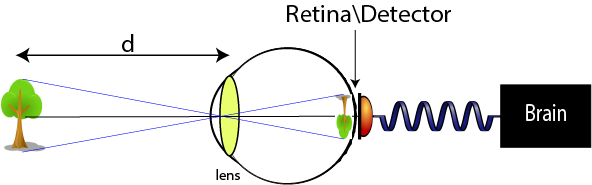
\includegraphics[width=0.65\textwidth]{Figures/eye.png}
 \caption{Eye seen as a Optical System, where $d$ is the distance between object and OS} 
\label{fig:eye}
\end{figure}


In order to take a photograph of an object, traditionally, we need to face a camera detector for example a CCD to the object, 
in a way similar to what we do when we point out our eyes to the objects we are seeing, Figure \ref{fig:eye}.
Both retina and camera record the spatial shape of the light that comes through.
This spatial information is necessary for the process of reconstructing an image of an object. 
It is important to point out that when using cameras we usually make images that are 2D representations of 3D objects. For this
reason we talk about an image plane, which is the plane where, depending on the OS, the 2D representation
of the object is going to be formed. 


What would happen if our retina or camera stopped recording the spatial shape of the light? if our retina now is 
only able to detect the light that reaches it, but not where it comes from, 
the imaging process would be imposible, since without spatial information it is not posible to create an image.
However, Two-photon imaging appears as a technique that allows to reconstruct images when spatial information of light is absent. 

Two-photon imaging started to draw attention after Pittman's first realisation \cite{pittman}. Figure \ref{fig:twoPh} depicts a scheme of the technique.
 A light source is divided into two paths. In one path the light is detected by a point like detector $D_A$
that is scanned in the transverse plane. In the other path a lens and an object are followed by a detector $D_B$ that erases the spatial information
 of the light.The two-photon image is retrieved by correlating the outputs of the detectors $D_A$ and $D_B$. 





\begin{figure}[h]
\centering
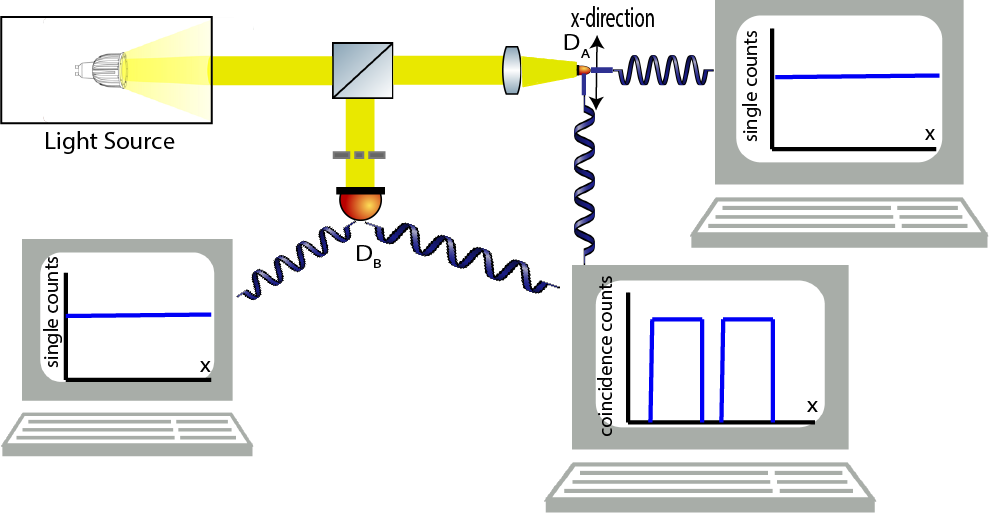
\includegraphics[width=0.75\textwidth]{Figures/twoPhotonSetup.png}
\caption{Two-photon imaging techniche setup} 
\label{fig:twoPh}
\end{figure}

There are different types of Two-photon imaging, and they differ from each other in the nature of the light 
source used. The first two-photon imaging realisation, obtained by Pittman in 1995\cite{pittman}, 
used entangled photon pairs as the light source. The second kind uses chaotic light. 
This light can be understood as the radiation coming from a blackbody at thermal equilibrium. 
Valencia \textit{et al.} where the first ones to present an experimental demonstration 
of two-photon ghost imaging with thermal-like sources\cite{thermalAlejandra}.

It is possible to reconstruct the image in this two experiments because there is some kind of 
correlation between the momentum of photons that are generated from the source. For the experiment with the quantum light source, the photons from a pair have negative momentum correlation.
In the experiment of the chaotic light, the pair of photons present a positive correlation\cite{positiveCorre}. 

Historically to study the effect of Two-photon imaging with different light sources was motivated by the question about the role of 
entanglement in the generation of the image. However, the role of different types of momentum correlations was not considered at that time. 
Recently Zhong \textit{et al.} presented a theoretical study of the effect of different types of momentum correlations on 
Two-photon imaging\cite{zhong}. In this monograph, we present an experiment in which it is possible to observe the effects of 
different types of momentum correlations on the generation of Two-photon imaging. We report preliminary results that pave the way for a more complete
study that will be \textit{pursued} by the Quantum Optics group.
 

In our experiment, we have done a Two-photon imaging in what is called a "lens-less two-photon image" configuration\cite{lensless}. We use a source of entangled 
photons to which it is possible to tune the transverse momentums
 correlations. The pair of photons are created by using the nonlinear optical process of spontaneous parametric down conversion (SPDC) in which 
a laser beam is focused into a nonlinear crystal, and occasionally pairs of photons are produced.  Interestingly, the geometry we used for the SPDC configuration
allows us to tune the momentum correlations by adjusting the waist of pump beam\cite{omar}.






This document is organized as follows: Chapter 2 presents a theoretical discussion about the fundamental 
aspects of the two-photon imaging, and the control of spatial correlations when using a SPDC source.  
In chapter 3 there is a meticulous explanation of the experimental setup used in this monograph, and its different steps.
The experimental results are presented in chapter 4 and finally, conclusions and perspectives are discussed on chapter 5.

